\section{Qualità di processo}
Per garantire la qualità dei \glo{processi} si utilizza come riferimento lo standard ISO/IEC 12207:1995. Dopo uno studio dettagliato di tale documento sono stati scelti i \glo{processi}
e le attività da utilizzare. Il tutto è stato semplificato ed adattato in base alle esigenze del progetto. Come è previsto nello standard, tutti i \glo{processi} e le attività sono raccolti 
nei \glo{processi}: primari, di supporto ed organizzativi. Le attività fanno parte a dei sotto \glo{processi} rispetto a quelli appena elencati e per questo motivo la loro 
appartenenza è resa chiara nella sezione: \glo{Processo} di riferimento.

\subsection{Processi primari}

\subsubsection{Analisi dei requisiti}
    \paragraph{Metrica - Percentuale requisiti obbligatori soddisfatti}
    \begin{itemize}
        \item \textbf{Codice:} MPC1
        \item \textbf{Descrizione:} È la percentuale dei requisiti che devono essere soddisfatti;
        \item \textbf{Processo di riferimento:} Sviluppo;
        \item \textbf{Sigla:} $PRS$
        \item \textbf{Formula:} $$PRS = {|requisiti \; soddisfatti| \over |requisiti \; totali|}\; \cdot \; 100$$
        \item \textbf{Range di valori che può assumere:}
        \begin{itemize}
            \item \textbf{Accettabile:} $PRS = 100\%$
            \item \textbf{Ottimale:} $PRS = 100\%$
        \end{itemize}
    \end{itemize} 
\subsubsection{Progettazione di dettaglio}
    \paragraph{Metrica - Incapsulamento CBO}
    \begin{itemize}
        \item \textbf{Codice:} MPC2
        \item \textbf{Descrizione:} Il "Coupling Between Objects" misura il numero delle classi correlate ad una classe in esame al di fuori dalla gerarchia di ereditarietà. Più è alto il grado di coupling della classe in esame e più il sistema è difficile da mantenere;
        \item \textbf{Processo di riferimento:} Sviluppo;
        \item \textbf{Sigla:} $CBO$
        \item \textbf{Formula:} $$CBO = {\sum_{i=1}^{N} C_i}$$
        con:
        \begin{itemize}
            \item $N$ = numero classi non appartenenti alla gerarchia di ereditarietà della classe in esame;
            \item $C_i$ =
            \begin{math} {
                \begin{cases}
                    1, & la \; $i$-esima \; classe \; \grave{e} \; correlata \; a \; quella \; in \; esame \\
                    0, & la \; $i$-esima \; classe \; non \; \grave{e} \; correlata \; a \; quella \; in \; esame
                \end{cases}
            }
            \end{math}
        \end{itemize}
        \item \textbf{Range di valori che può assumere:}
        \begin{itemize}
            \item \textbf{Accettabile:} $0 \leq{} CBO \leq 4$
            \item \textbf{Ottimale:} $0 \leq{} CBO \leq 2$
        \end{itemize}
    \end{itemize}

    \paragraph{Metrica - Livello profondità gerarchia}
    \begin{itemize}
        \item \textbf{Codice:} MPC3
        \item \textbf{Descrizione:} È il valore intero che indica la profondità della gerarchia formata tra classi. Se una gerarchia è formata da una classe allora il valore è uguale a 1;
        \item \textbf{Processo di riferimento:} Sviluppo;
        \item \textbf{Sigla:} $LPG$
        \item \textbf{Range di valori che può assumere:}
        \begin{itemize}
            \item \textbf{Accettabile:} $1 \leq{} LPG \leq 3$
            \item \textbf{Ottimale:} $1 \leq{} LPG \leq 2$
        \end{itemize}
    \end{itemize}

\subsubsection{Codifica}  
    \paragraph{Metrica - Numero di parametri per metodo} 
    \begin{itemize}
        \item \textbf{Codice:} MPC4
        \item \textbf{Descrizione:} Un numero elevato di parametri per metodo può indicare il bisogno di ridurre funzionalità associate a tale metodo. Più è grande questo valore e più la possibilità aumenta nel commettere errori progettuali;
        \item \textbf{Processo di riferimento:} Sviluppo;
        \item \textbf{Sigla:} $NPM$
        \item \textbf{Range di valori che può assumere:}
        \begin{itemize}
            \item \textbf{Accettabile:} $0 \leq{} NPM \leq 8$
            \item \textbf{Ottimale:} $0 \leq{} NPM \leq 4$
        \end{itemize}
    \end{itemize}

    \paragraph{Metrica - Linee di commento per linee di codice}
    \begin{itemize}
        \item \textbf{Codice:} MPC5
        \item \textbf{Descrizione:} È il rapporto tra linee di commento e linee di codice. Per le linee di codice si intende Logical SLOC il numero di linee di codice effettive che corrispondono al numero di statement;
        \item \textbf{Processo di riferimento:} Sviluppo;
        \item \textbf{Sigla:} $LCLC$
        \item \textbf{Formula:}$$LCLC = {|linee \; di \; commento| \over |linee \; di \; codice|}$$
        \item \textbf{Range di valori che può assumere:}
        \begin{itemize}
            \item \textbf{Accettabile:} $LCLC \geq 0.25$
            \item \textbf{Ottimale:} $LCLC \geq 0.30$
        \end{itemize}
    \end{itemize}

\subsection{Processi supporto}

\subsubsection{Implementazione}
    \paragraph{Metrica - Indice di Gulpease}
    \begin{itemize}
        \item \textbf{Codice:} MPC6
        \item \textbf{Descrizione:} È l'indice di leggibilità di un determinato testo. Calcola la lunghezza delle parole e delle frasi rispetto al numero totale delle lettere. Il valore è un intero da 0 a 100; se esso è inferiore a 80 sarà difficile da leggere per chi ha la licenza elementare, mentre se è inferiore a 40 sarà difficili da leggere per chi ha un diploma superiore;
        \item \textbf{Processo di riferimento:} Documentazione;
        \item \textbf{Sigla:} $IG$
        \item \textbf{Formula:} $$IG = 89 + {{300 \; \cdot \; |frasi| \; - \; 10 \; \cdot \; |lettere|}\over |parole|}$$
        \item \textbf{Range di valori che può assumere:}
        \begin{itemize}
            \item \textbf{Accettabile:} $40 < IG < 100$
            \item \textbf{Ottimale:} $80 < IG < 100$
        \end{itemize}
    \end{itemize}

\subsubsection{Verifica}
    \paragraph{Metrica - Code coverage}
    \begin{itemize}
        \item \textbf{Codice:} MPC7
        \item \textbf{Descrizione:} È la percentuale di copertura del codice attraversato dai test rispetto al totale del codice di base. Per dare una misurazione in termini di grandezza si adoperano le linee di codice come riferimento;
        \item \textbf{Processo di riferimento:} \glo{Processi} di verifica;
        \item \textbf{Sigla:} $CC$
        \item \textbf{Formula:} $$CC = {|linee \; di \; codice \; percorse \; dai  \; test| \over |linee \; di \; codice \; totali|} \; \cdot \; 100$$
        \item \textbf{Range di valori che può assumere:}
        \begin{itemize}
            \item \textbf{Accettabile:} $CC = 80\%$
            \item \textbf{Ottimale:} $CC = 100\%$
        \end{itemize}
    \end{itemize}

\subsection{Processi organizzativi}

\subsubsection{Pianificazione}
    \paragraph{Metrica - Schedule variance}
    \begin{itemize}
        \item \textbf{Codice:} MPC8
        \item \textbf{Descrizione:} È il valore che indica se si è in linea ($=0$), in anticipo ($>0$) oppure in ritardo ($<0$) rispetto alla schedulazione delle attività di progetto pianificate nella \glo{baseline};
        \item \textbf{Processo di riferimento:} Gestione;
        \item \textbf{Sigla:} $SV$
        \item \textbf{Formula:} $$SV = {BCWP \; - \; BCWS}$$
        con:
        \begin{itemize}
            \item $BCWP$ = Budgeted Cost of Work Performed (valore delle attività eseguite nella data corrente);
            \item $BCWS$ = Budgeted Cost of Work Scheduled (costo pianificato per la realizzazione delle attività di progetto alla data corrente);
        \end{itemize}
        \item \textbf{Range di valori che può assumere:}
        \begin{itemize}
            \item \textbf{Accettabile:} $SV = 0$
            \item \textbf{Ottimale:} $SV > 0$
        \end{itemize}
    \end{itemize}

    \paragraph{Metrica - Budget variance}
        \begin{itemize}
            \item \textbf{Codice:} MPC9
            \item \textbf{Descrizione:} È il valore che indica se alla data corrente si è speso di più ($>0$) o di meno ($<0$) rispetto a quanto pianificato dal budget totale $B_{tot}$;
            \item \textbf{Processo di riferimento:} Gestione;
            \item \textbf{Sigla:} $BV$
            \item \textbf{Formula:} $$BV = {BCWS \; - \; ACWP}$$
            con:
            \begin{itemize}
                \item $BCWS$ = Budgeted Cost of Work Scheduled (costo pianificato per la realizzazione delle attività di progetto alla data corrente);
                \item $ACWP$ = Actual Cost of Work Performed (costo effettivamente sostenuto alla data corrente);
                \item $B_{tot}$ = Budget totale.
            \end{itemize}
            \item \textbf{Range di valori che può assumere:}
            \begin{itemize}
                \item \textbf{Accettabile:} $0 \leq BV < ACWP$
                \item \textbf{Ottimale:} $0 \leq BV \leq B_{tot}$
            \end{itemize}
        \end{itemize}

\newpage %adattamento pagina

    \rowcolors{2}{grigetto}{white}
    \renewcommand{\arraystretch}{1.5}
    \begin{longtable}{ c C{4cm} c c c}
    \caption{Tabella metriche dei processi}\\
    \rowcolor{darkblue}
    \textcolor{white}{\textbf{Metrica}} & \textcolor{white}{\textbf{Nome}} & \textcolor{white}{\textbf{Sigla}} & \textcolor{white}{\textbf{Range Accettabile}} & \textcolor{white}{\textbf{Range Ottimale}}\\
    MPC1 & Percentuale Requisiti Soddisfatti & $PRS$ & $PRS = 100\%$ & $PRS = 100\%$ \\
    MPC2 & Coupling Between Objects & $CBO$ & $0 \leq CBO \leq 4$ & $0 \leq CBO \leq 2$ \\
    MPC3 & Livello Profondità Gerarchia & $LPG$ &  $1 \leq LPG \leq 3$ &  $1 \leq LPG \leq 2$ \\
    MPC4 & Numero di Parametri per Metodo & $NPM$ & $0 < NPM < 8$ & $ 0 < NPM < 4$ \\
    MPC5 & Linee di Codice per Linee di Commento & $LCLC$ & $LCLC \geq 0.25$ & $LCLC \geq 0.30$ \\
    MPC6 & Indice di Gulpease & $IG$ & $40 < IG < 100$ & $80 < IG < 100$ \\
    MPC7 & Code Coverage & $CC$ & $CC = 80\%$ & $CC = 100\%$  \\
    MPC8 & Schedule Variance & $SV$ & $SV = 0$ & $SV > 0$  \\	
    MPC9 & Budget Variance & $BV$ & $0 \leq BV < ACWP$ & $0 \leq BV \leq B_{tot}$  \\
    \end{longtable}

\subsection{Ciclo di Deming}
Il ciclo di Deming è un metodo di gestione iterativo per il controllo e il miglioramento continuo dei processi (e anche dei prodotti) suddiviso in 4 fasi: Plan, Do, Check e Act. 
Anche la norma ISO/IEC 12207 utilizza questo ciclo per scopi di miglioria dei \glo{processi}. Per garantire la qualità dei \glo{processi} e la coerenza allo standard, il gruppo \Gruppo  
ha scelto di adottare il ciclo PDCA.

\begin{figure}[h]
    \centering
    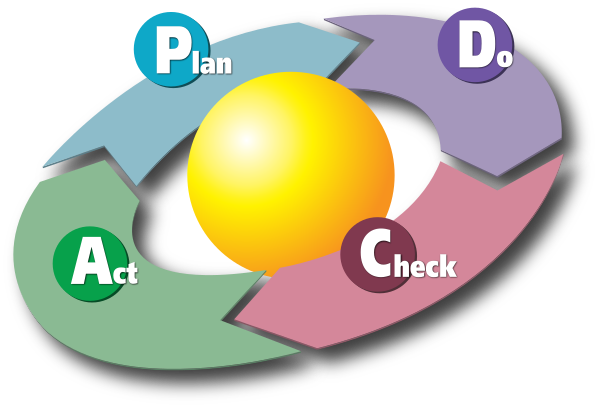
\includegraphics[scale=0.2]{Sezioni/Immagini/PDCA.png}
    \caption{Ciclo PDCA - Plan Do Check Act}
\end{figure}

\textbf{Fasi del ciclo PDCA:}
\begin{itemize}
    \item \textbf{Plan}: Definisce attività e scadenze necessarie al raggiungimento dei specifici obiettivi di miglioramento;
    \item \textbf{Do}: Esegue le attività di "Plan";
    \item \textbf{Check}: Verifica l'esito delle azioni di miglioramento rispetto alle attese. Si analizzano i risultati del "Do" e li si confrontano con gli obiettivi individuati nel "Plan";
    \item \textbf{Act}: Consolida il tutto e cerca dei metodi per il prossimo miglioramento. Se il "Check" ha dimostrato che il "Plan" implementato dal "Do" è migliore rispetto ai precedenti \glo{processi} standard, allora questo piano diventa il nuovo \glo{processo} standard. Altrimenti il vecchio standard in uso rimarrà la \glo{baseline}.
\end{itemize}